\section{Introduction}
\label{sec:intro}

Software is ubiquitous. With applications targeting a diverse set of
environments and platforms, developers commonly turn to automated testing with
the hope of preventing defects. Tests exercise a program over its input domain
to validate its functionality on that input or fail. Ideally, tests are
deterministic: they either always pass or always fail. In the case of regression
testing, each test allows a developer to make changes --- functional or
otherwise --- to the code under test with the confidence that existing behaviour
will not be modified. During feature development, tests have a similar benefit.
A passing test confirms that a new feature is behaving correctly. Test suites
are run regularly as part of the development cycle; unintended behaviour is
brought to the developer's attention by one or more failing tests. Despite their
benefits, automated tests are ultimately just more software, and just as
software is rarely bug free, automated tests are often plagued with bugs of
their own --- they are not always deterministic.

An intermittently failing automated test that fails often enough can be made
effectively deterministic with iteration so long as it is cheap. We call those
that are expensive or rarely fail \emph{flaky} tests.

Environmental factors are often related to intermittent test failure. The
further we travel up the layers of automated testing toward the system level,
the more environmental factors we introduce. Unit tests target and exercise
isolated sections of code. A well written unit test's outcome is almost
guaranteed to depend only on the behaviour of the code it exercises. Integration
tests may depend on an external service (\eg, a database), so may sometimes fail
unexpectedly. Most vulnerable are acceptance tests. Since they run on a complete
system, they are potentially open to interference by any number of environmental
events or characteristics. For example, an operating system starved of memory
could kill the application, or, a particularly slow start-up time could cause a
timeout to occur.

\subsection{\Flaky Tests are a Real Problem}

\Flaky tests are no small issue. Mozilla\cite{mozillaFlakyTestBug} and Chromium
have known flaky tests. Android even includes an {\tt @FlakyTest}
annotation\cite{androidFlakyInterface} in its testing kit for automatic re-
running of known \flaky tests. The {\tt @FlakyTest} Android annotation has been
present since the initial release of Android.

When the latest changes are due to be released, the \flaky tests must be
considered. Normally, a particular software iteration would be held back until
all tests pass, but with \flaky tests thrown into the mix - it may take multiple
runs before all the tests pass at once - again, adding overhead.

The set of \flaky tests causes confusion, obscures real failures and erodes
trust.

Simply surpressing the \flaky tests is not a long-term solution. Informally, let
a valid test be a test that asserts that some unit of the application behaves as
expected. A redundant test might check behaviour that is not required, or is
tested thoroughly elsewhere. Assuming all tests in a suite are valid, then any
\flaky tests in the suite are also valid. A \flaky test may cover behaviour that
is not tested elsewhere. Suppressing (temporarily retiring) the \flaky test may
do more harm than good, since the behaviour it previously tested will now be go
completely unchecked unless manually tested upon each commit.

\subsection{Automating the Diagnostic Process}

Our goal is to automate as much of the process for fixing a flaky test as
possible, freeing developers to spend time developing the software, rather than
debugging tests that are in fact intended to speed up the development process.
Ultimately, each test case must be investigated and fixed by a developer, but as
we will show, much of the legwork can be automated.

The tool we propose --- \textit{\venera} --- gathers and analyses information
much in the same way as a developer would. First, it identifies the flaky tests
in a test suite. Then, it employs techniques similar to those discussed by
\citet{ArumugaNainar:2010:ABI:1806799.1806839} to gather relevant debugging
information over a series of test runs. Finally we analyze the gathered data and
identify predicates strongly associated with test failure. Our tool takes
advantage of the continuous integration environment, gathering data each time an
associated test suite is run. Figure \ref{fig:developer_workflow} shows a high-
level \venera workflow.

Previous and potential future work with an industry software startup lead us to
target the Android platform for our proof of concept.

\begin{figure}[h]

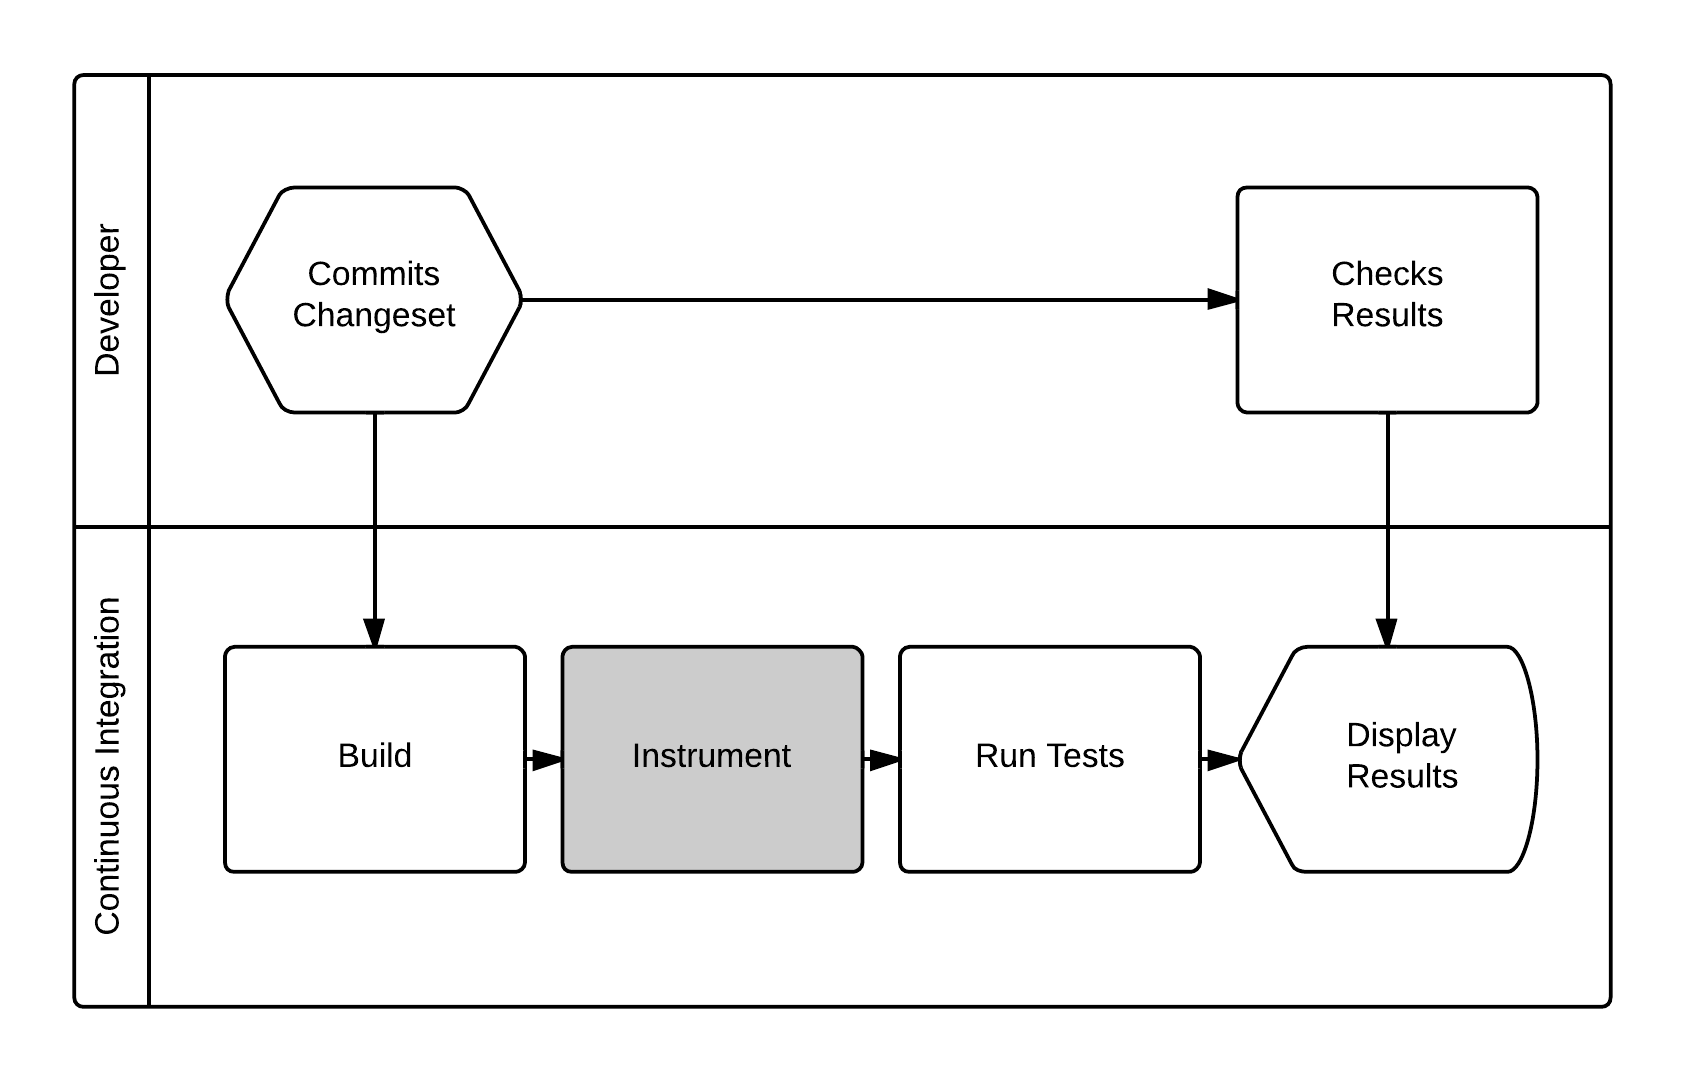
\includegraphics[width=\linewidth]{Images/developer_workflow}

\caption{}
\label{fig:developer_workflow}
\end{figure}

Running as a continuous integration step is a natural application. For one, test
suites are run as continuous integration steps themselves. In addition, we want
to be as transparent as possible.

One of the primary initial goals of the project was to create a continuous
integration plugin to present the data gathered during the identification of the
\flaky tests. As we researched the area, we realised that the indentification of
\flaky tests is the most well-covered and least interesting area. The more
experimental and relatively untouched area dealing with adaptive instrumentation
and analysis of collected information eventually became our primary focus.

Reaching a stage where we could analyze the gathered data proved to be far more
challenging than expected. The relative youth of the Android platform was a
clear stumbling block, since tried and tested instrumentation tools in the world
of the Java Virtual Machine had only just begun to acknowledge their Dalvik
sibling. As such, we document and discuss many of our design decisions along the
way.

\Flaky tests are hard to reproduce. In general, there are three stages during
which we may intervene:
\begin{enumerate}
	\item Identification - which tests in the suite are flaky?
	\item Prioritisation - which of the \flaky tests should we fix first?
	\item Resolution - what information can we gather to speed the resolution of a test?
\end{enumerate}

Ultimately, the final stage is the target. In order to tackle the problem
practically, knowledge gathered at each stage must be combined and considered.

Existing tools provide answers to 1. This information can be used to inform
manual inspection of 2. As of yet, no tool exists to tackle 3.

In a typical software development project, continuous integration systems will
be set up from the beginning. Developers write code and commit to source
control. A master server will detect the change and assign one of a number of
build agents (other servers with the capability to build the project(s) -
virtual or otherwise) an attached job.

For a typical job, the chosen build agent pulls down the latest changes,
compiles and runs the tests and runs any post-build tasks. At the end, any build
artifacts (distributable packages, test results, etc.) will be uploaded to the
master server and the agent will be once again free to build the next iteration.
Note that in reality, a job can comprise of any number of runnable steps - from
executing a shell script to hitting an external server.

It is obvious that, if we are to develop a tool to assist developers with \flaky
tests, we should run as part of a modular continuous integration system.

The rest of the report will proceed with a familiar structure.
\autoref{sec:context} describes the theory and context behind the project.
\autoref{sec:example} presents a motivating example of a \flaky test. Following
the example, we detail our general approach in \autoref{sec:approach}.
\autoref{sec:imp} discusses the design and of our proof of concept tool,
\venera. Finally, \autoref{sec:relwork} compares our work to that of previous
research and tools. We wrap up with a conclusion (\autoref{sec:conc}) and
suggest future directions for both \venera and the research in general.
